\FloatBarrier%
\section{CSPH}
\label{sec:csph}

We model the collision between elastic solids using a penalty-based contact
force model. A contact force based approach for collision handling will
eliminate the spurious interaction between bodies, which occurs while modeling
with an SPH-based model. The contact force model follows the work of
\cite{mohseni2021particle}.

\subsection{Discrete governing equations}
\label{sec:discrete-governing-equations}
The governing equations of including the new contact force term are:
\begin{equation}
\label{eqn:sph-continuity}
  \frac{\tilde{d}\rho_a}{dt} = \sum_{b \in A} \; \frac{m_b}{\rho_{b}} \; (
  \rho_{a} \; \tilde{\ten{u}}_{ab} \; + \;
  (\rho \; (\tilde{\ten{u}} \; - \;
  \ten{u}))_{ab}) \; \cdot \nabla_{a} W_{ab},
\end{equation}
\begin{equation}
\label{eqn:sph-momentum}
  \frac{\tilde{d}\ten{u}_{a}}{dt} = - \sum_{b \in A} m_b \bigg[
  \bigg(\frac{p_a}{\rho_a^2} + \frac{p_b}{\rho_b^2}\bigg) \ten{I} -
  \bigg(\frac{\teng{\sigma}^{'}_{a}}{\rho_a^2} +
  \frac{\teng{\sigma}^{'}_{b}}{\rho_b^2} + \Pi_{ab} \ten{I} \bigg) \bigg]  \cdot \nabla_{a} W_{ab} +
  \ten{g}_{a} + \frac{1}{m_a}\sum_{b \in B} \ten{F}^{\text{cont}}_{a \leftarrow b}.
\end{equation}
Here, $\ten{F}^{cont}_{a}$ is the force acting on particle $a$ due to
\begin{figure}[!htpb]
  \centering
  \includegraphics[width=1.0\textwidth]{images/csph/images/contact_force/contact_force_description}
  \caption{Bodies under collision which are divided into primary and
    secondary.}
\label{fig:bodies_under_collision}
\end{figure}
contact with the other elastic bodies which will be discussed in
\cref{sec:contact-algorithm}.

\FloatBarrier%
\section{Contact algorithm}
\label{sec:contact-algorithm}
In the current work we have utilized the contact force model proposed by
\cite{mohseni2021particle}. The force acting on a particle $a$ of body A due
to the interaction with the particles of body $B$ can be resolved into a
normal and tangential component. The normal force component is utilised to
make sure that the particles of different bodies do not penetrate into each
other, while the tangential component is used to model the friction between
the interacting solids. According to \cite{mohseni2021particle}, we divide the
bodies under interaction into primary and secondary bodies, as shown in
\cref{fig:bodies_under_collision}.
% In usual DEM to compute the force on particle i of body A, the force is
% computed by considering the overlap of particle i with each and every
% particle of body j by considering the particle j to be spherical. This leads
% to unphysical modeling of contact force when the body is interacting with a
% flat surface or surfaces which are not spherical by nature. The current
% contact force is surface aware. The force on particle $i$ is computed by
% equation
The normal force ($\teng{F}_a^{n}$) on
particle $a$ due to the interaction with the particles $b$ of body $B$ is
computed as,
\begin{equation}
  \label{eq:contact-algorithm-normal}
  \ten{F}_a^n = k_r \delta_{n^{c}}^{a} \ten{n}_a^{c}.
\end{equation}
Here, the overlap $\delta_{n^{c}}^{a}$ is computed using
\begin{equation}
  \label{eq:csph:cf-overlap}
  \delta_{n^{c}}^{a} = \Delta x - d_a,
\end{equation}
where,
\begin{equation}
  \label{eq:cf-distance-computation}
  d_a = \frac{
    \displaystyle\sum\limits_{b = 1}^{\text{NP}^{b}} \;
    \big( \ten{n}_a^{c} \cdot \ten{r}_{ab} \big)  \frac{m_b}{\rho_b} W_{ab}}
  {
    \displaystyle\sum\limits_{b = 1}^{\text{NP}^{b}} \;
    \frac{m_b}{\rho_b} W_{ab}},
\end{equation}
and the normal contact vector $\ten{n}_a^{c}$ is computed using
\begin{equation}
  \label{eq:cf-normal-vector}
  \ten{\hat{n}}_a^{c} = \frac{
    \displaystyle\sum\limits_{b = 1}^{\text{NP}^{b}} \;
    \frac{\ten{r}_{ab}}{r_{ab}}  \frac{m_b}{\rho_b} W_{ab}}
  {
    \displaystyle\sum\limits_{b = 1}^{\text{NP}^{b}} \;
    \frac{m_b}{\rho_b} W_{ab}},
\end{equation}
\begin{equation}
  \label{eq:cf-normal-vector}
  \ten{n}_a^{c} = \frac{\teng{\hat{n}}_a^{c}}{||\teng{\hat{n}}_a^{c}||}.
\end{equation}
\begin{figure}[!htpb]
  \centering
  \includegraphics[width=0.3\textwidth]{images/csph/images/contact_force/contact_force_delta_computation}
  \caption{Pictorial representation of distance between a particle and a body.}
\label{fig:contact_force_delta_computation}
\end{figure}
Where $\Delta x$ being the initial spacing between the particles, $k_r$ is the
normal spring stiffness coefficient. \Cref{fig:contact_force_delta_computation}
shows $\Delta x$ and $d_a$ quantities, respectively. Note that while computing
the overlap of particle $a$ with the body $B$ we have computed an effective
overlap, rather than per particle interaction. This is effectively able to model
the interaction between non-smooth surfaces in contrast with particle-particle
force computation.

\subsection{Tangential force computation}
\label{sec:tangential-force-computation}
We associate a tangential spring attached to particle $a$
($|\Delta \textit{\textbf{l}}_a|$) and body $B$ to compute the tangential force
($\ten{F}_{a}^{t}$), which initially has a magnitude of zero
($|\Delta \textit{\textbf{l}}_a|=0$). The tangential spring is activated when
the particle comes into contact with body $B$. The tangential force is
history-dependent. The contact friction force is proportional to the tangential
spring displacement, which is integrated over the contact time as
\begin{equation}
  \label{eq:tangential-force}
  \ten{F}_{a}^{t^{n+1}} =
  -k_f \Delta \textit{\textbf{l}}_a^{\,n + 1} =
  -k_f \big[\big(\Delta {\textit{\textbf{l}}}_a^{\,n} \
  + \ten{v}_{ab}^{n + 1} \Delta t\big) \cdot \ten{t}_a^{n + 1} \big] \
  \ten{t}_a^{n + 1},
\end{equation}
where $\Delta t$ is the time step, $\ten{v}_{ab} = \ten{v}_{a} - \ten{v}_b$ is
the relative velocity of the primary particle $a$ with respect to the closest
secondary particle $b$, $\ten{t}_a$ is the tangential unit vector, and $k_f$ is the tangential spring stiffness
coefficient. Here, $n$ and $n+1$ represent the times which are $\Delta t$ apart.
The tangential unit vector is computed by,
\begin{equation}
  \label{eq:tangential-vect}
  \ten{t}_a = \frac{\ten{v}_{ab} - (\ten{v}_{ab} \cdot \ten{n}_a^{c}) \ten{n}_a^{c}}{|\ten{v}_{ab} - (\ten{v}_{ab} \cdot \ten{n}_a^{c}) \ten{n}_a^{c}|}.
\end{equation}

The tangential force is coupled to the normal force through the Coulomb's law,
\begin{equation}
  \label{eq:Coulomb-law}
  \ten{F}_{a}^{t} = \min(\mu |\ten{F}_{a}^{n}|, |\ten{F}_{a}^{t}|) \
  \frac{\ten{F}_{a}^{t}}{|\ten{F}_{a}^{t}|}.
\end{equation}
This allows us to impose the sliding friction condition between the
interacting solids. Finally, the total force acting on the particle $a$ due to
the interaction with body $B$ is:
\begin{equation}
  \label{eq:contact-force}
  \ten{F}_{a}^{\text{cont}} = \ten{F}_{a}^{n} + \ten{F}_{a}^{t}
\end{equation}

\begin{figure}[!htpb]
  \centering
  \includegraphics[width=0.3\textwidth]{images/csph/images/contact_force/contact_force_description_3}
  \caption{Force transfer to the secondary particles $b$ from the primary body particle $a$}
\label{fig:secondary_particle_contact_foce_transfer}
\end{figure}
An equal and opposite force of the same magnitude is applied to the closest
secondary particle $b$ of $a$ as shown in
\cref{fig:secondary_particle_contact_foce_transfer},
\begin{equation}
  \label{eq:contact-force}
  \ten{F}_{b}^{\text{cont}} = - \ten{F}_{a}^{\text{cont}}.
\end{equation}

% =========================================== %
% ------ Results start ---------------------- %
% =========================================== %

\FloatBarrier%
\subsection{Stress wave propagation in granular media}
\label{sec:results-stress-wave-propagation-with-friction}
\begin{figure}[!htpb]
  \centering
  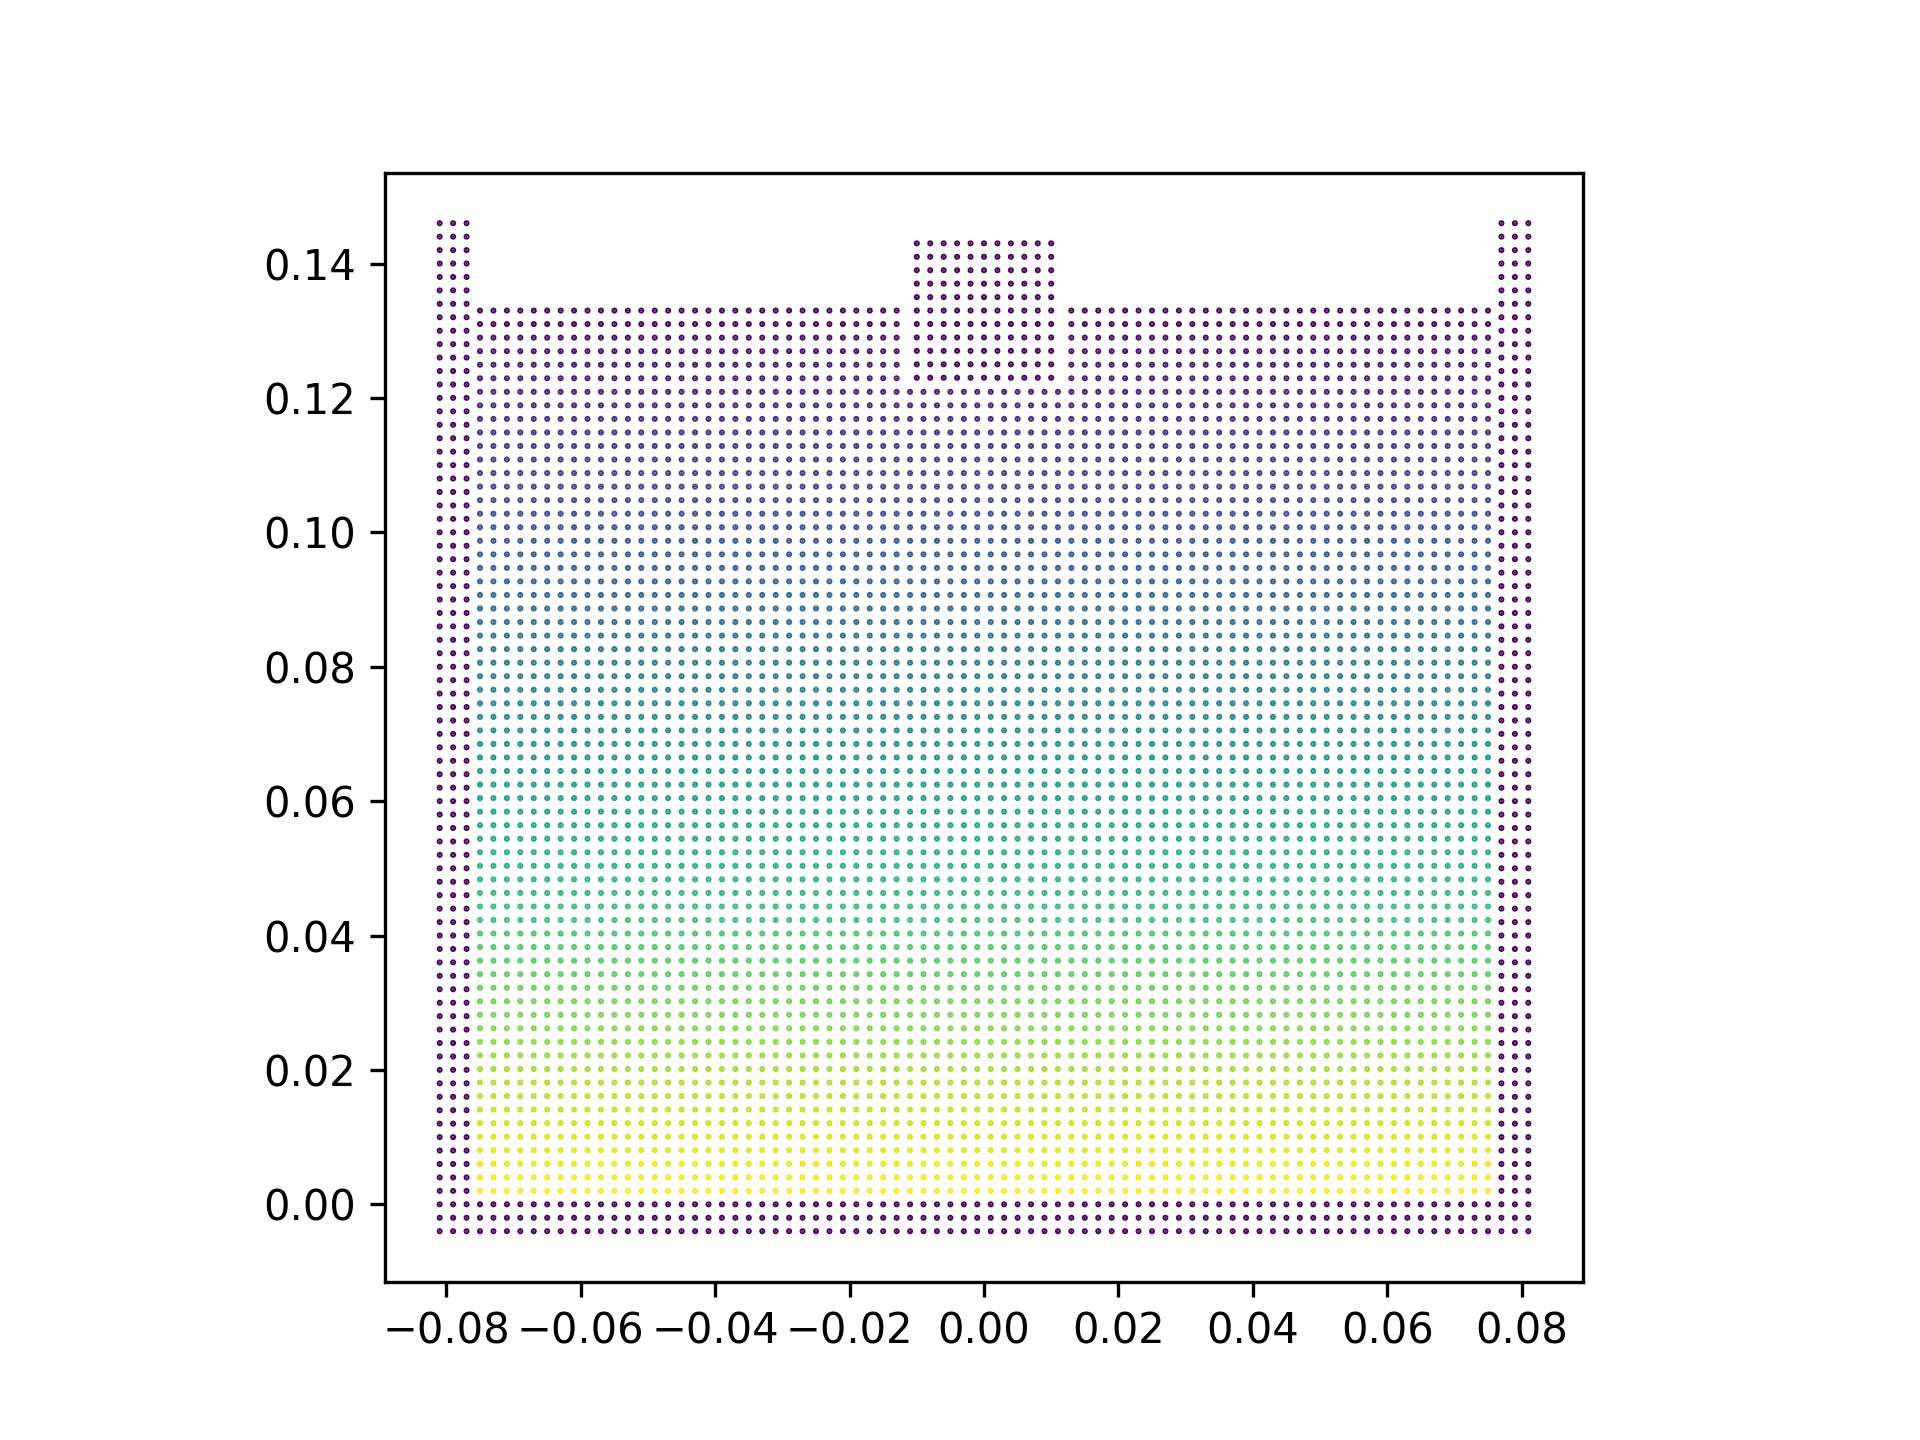
\includegraphics[width=1.0\textwidth]{images/csph/images/de_2021_stress_wave_in_granular_material_part_2/schematic}
  \caption{Schematic of the initial placement of the frictional granular media including the impactor and walls}
\label{fig:results-stress-wave-propagation-part-II}
\end{figure}
The elastic wave propagation in a granular media is carried out, and whose
experimental study was executed by \cite{guilkey2001improved}. We consider five
identical disks placed at an angle of $45$ degrees, allowed to be impacted by a
moving wall from right with a velocity $5.6$ m\,s\textsuperscript{-1} in
horizontal direction as depicted in
\cref{fig:results-stress-wave-propagation-part-II}. Each granular disk has a
radius of $50$ mm, which are initially placed such that they are just touching.
The rigid box are modelled as rigid surfaces. The material parameters of
the disc as well as the numerical parameters used in the numerical simulation
are listed in \cref{tab:de-stress-part-2-params}.
\begin{table}[!ht]
  \centering
  \begin{tabular}[!ht]{ll}
    \toprule
    Quantity & Values\\
    \midrule
    $K$, Bulk modulus & $102$ GPa \\
    $G$, Shear modulus & $72$ GPa \\
    $\rho$, density & $1900$ kg\,m\textsuperscript{-3} \\
    gravity $[g_x, g_y, g_z]$ & $[0.0, 0.0, 0.0]$\\
    $k_r$, Normal stiffness coefficient & $1.75 \times 10^{11}$ \\
    $k_f$, Tangential stiffness coefficient & $5 \times 10^{10}$ \\
    $\mu$, Friction coefficient & 0.5 \\
    \bottomrule
  \end{tabular}
  \caption{Material and numerical parameters used for the stress wave propagation problem.}%
  \label{tab:de-stress-part-2-params}
\end{table}
\Cref{fig:de-stress-wave-compare} shows the particle plots of the granular
discs with the stress fringes from the experiment \citep{guilkey2001improved},
and the simulation carried in the present study, and from the numerical study
of \cite{de2021modelling}, where the simulation is carried out using a total
Lagrangian material point method (TLMPM). The snapshots of the current work
are taken at time $0.2$ ms, while the results of experimental and TLMPM result
correspond to the time at $0.12$ ms. This is due to the initial placement of
the discs in the current work and the stress fringes being sensitive to
initial placement.
\begin{figure}[!htpb]
  \centering
  \begin{subfigure}{1.0\textwidth}
    \centering
    \includegraphics[width=0.7\textwidth]{images/csph/images/de_2021_stress_wave_in_granular_material_part_2/bardenhagen_2001}
    \subcaption{}\label{fig:de-stress-wave-bardenhagen}
  \end{subfigure}

  \begin{subfigure}{1.0\textwidth}
    \centering
    \includegraphics[width=0.7\textwidth]{images/csph/images/de_2021_stress_wave_in_granular_material_part_2/tlmpm_2021}
    \subcaption{}\label{}
  \end{subfigure}

  \begin{subfigure}{1.0\textwidth}
    \centering
    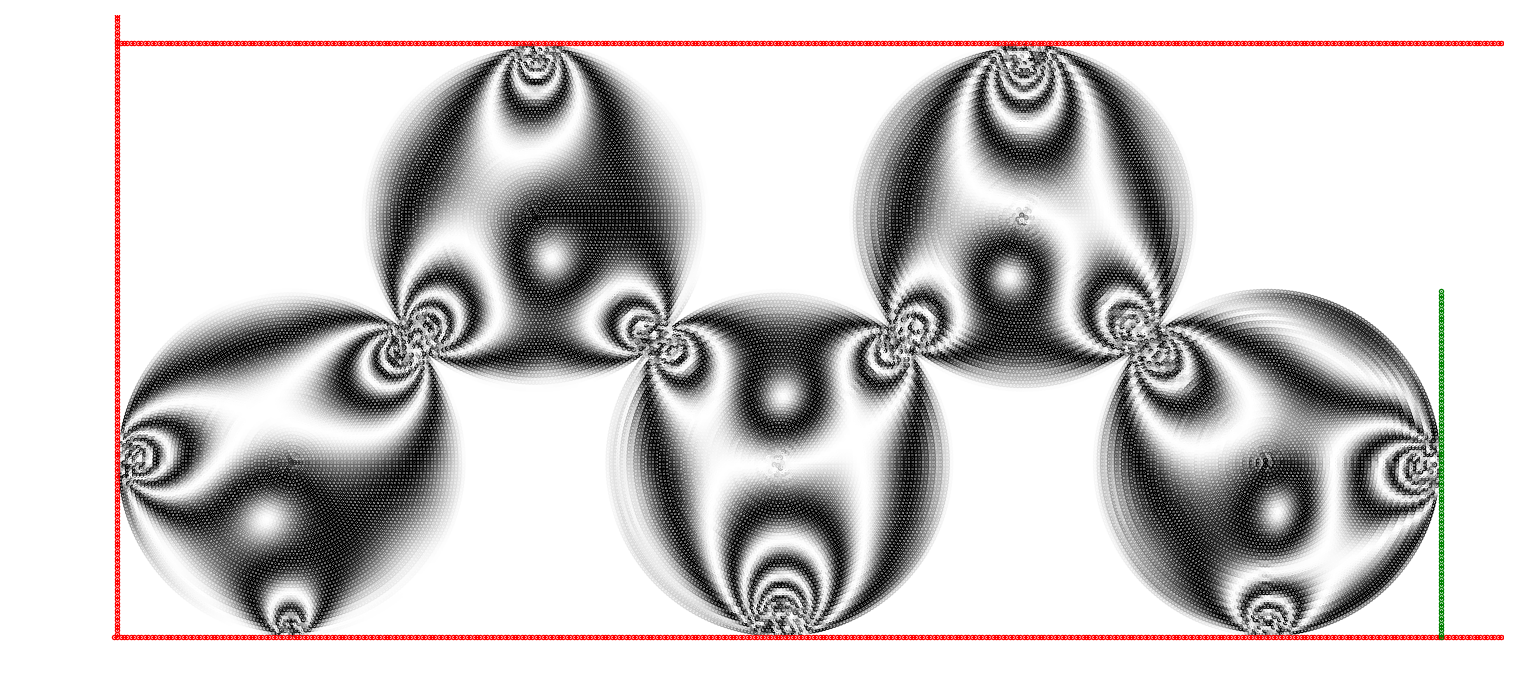
\includegraphics[width=0.8\textwidth]{figures/csph/figures/de_2021_stress_wave_in_granular_material_part_2/case_mohseni/time0}
    \subcaption{}\label{fig:de-stress-wave-current}
  \end{subfigure}
  \caption{Stress fringes of the granular discs from (a) experiment
    \citep{guilkey2001improved}, (b) TLMPM \citep{de2021modelling} (c) Current work}
\label{fig:de-stress-wave-compare}
\end{figure}
